\documentclass{scrartcl}

\usepackage{german}
\usepackage[utf8]{inputenc}  %Umlaute
\usepackage[T1]{fontenc}     %Umlauttrennung
\usepackage{lmodern}         %modernes Schriftbild
\usepackage{amsmath}         %math Umgebungen
\usepackage{graphicx}
\usepackage{hyperref}        %URLs
\usepackage{gensymb}         %Gradzeichen
\usepackage{float}           %Positionierung von Tabellen und Abb
\usepackage{textgreek}


\begin{document}
\begin{titlepage}
  \begin{center}
    \vspace*{1cm}
    \LARGE
    Physikpraktikum für Naturwissenschaftler \\
    \vspace*{1cm}
    \Huge
    \textbf{Versuch: Wechselstromkreise} \\
    \vspace*{0.3cm}
    \Large
    Durchgeführt am 10. Januar 2019 \\
    Betreuer: David Reinhardt \\
    \vspace*{2.5cm}
    Gruppe 13 \\
    Felix Burr: felix.burr@uni-ulm.de \\
    Johannes Spindler: johannes.spindler@uni-ulm.de \\
    \vfill 
  \end{center}
  Wir bestätigen hiermit, das Protokoll selbstständig erarbeitet zu haben und in genauer Kenntnis über dessen Inhalt zu sein. \\
  \vspace*{0.8cm}
  \\
  Felix Burr
  \hfill
  Johannes Spindler
\end{titlepage}
\pagebreak
\tableofcontents


\pagebreak

\section{Einleitung}
Aus dem Ohm'schen Gesetz ist der elektrische Widerstand $R$ als konstantes Verhältnis der Spannung $U$ zur Stromstärke $I$ bekannt:
\begin{align}
R = \frac{U(t)}{I(t)} = const
\end{align}
Das gilt für Gleich- wie Wechselspannungen, allerdings spricht man bei Wechselstromkreisen vom Scheinwiderstand $|Z|$, der als Betrag der (komplexwertigen) Impedanz $Z$ definiert ist:
\begin{align}
|Z| = \frac{U_{0}}{I_{0}}
\end{align}
$U_{0}$ und $I_{0}$ bezeichnen die Amplitudenwerte von Spannung und Stromstärke.

Die Impedanz eines Zweipols fasst im Realteil den Wirkwiderstand $R$ und im Imaginärteil den Blindwiderstand $X$ zusammen. Während beim Wirkwiderstand die Sinuskurven von Spannung und Strom phasengleich sind, liegt beim Blindwiderstand eine Phasenverschiebung von +90\degree oder -90\degree vor. Diese Phasenverschiebung ist der Grund, warum Wirk- und Blindwiderstände einer Schaltung nicht einfach zu einem Gesamtwiderstand addiert werden dürfen, sondern als komplexwertige Impedanz $Z$ verstanden werden. 

Vektoriell betrachtet ist $Z$ ein Vektor mit einer $R$-Komponente auf der x-Achse und einer $X$-Komponente auf der y-Achse. Dann ist der Winkel $\varphi$ zwischen x-Achse und $Z$ der Phasenwinkel und die Länge $|Z|$ des Vektors der Scheinwiderstand.

Im ersten Versuch wird der Scheinwiderstand $|Z|$ für einen Widerstand, einen Kondensator und eine Spule bestimmt. Im zweiten Versuch sollen Impedanz und Phasenverschiebung eines unbekannten Zweipols bestimmt werden und mit den Theoriewerten verglichen werden.
\section{Impedanzmessung an Widerstand, Kondensator und Spule}
\subsection{Versuchsaufbau und Durchführung}
Der zu messende Zweipol wird wie in Abbildung \ref{fig:Aufbau} mit einem bekannten Widerstand $R_{I}$, der zur Bestimmung von $I$ dient, in Reihe geschaltet und an einen Frequenzgenerator und ein Oszilloskop angeschlossen. Als Frequenz wird für Widerstand und Kondensator $f = 1kHz$ und für die Spule $f = 10kHz$ gewählt. Auf Kanal 1 des Oszilloskops wird die Amplitude $U_{1}$ der am Zweipol anliegenden Spannung und auf Kanal 2 die Amplitude $U_{2}$ der an R\textsubscript{I} anliegenden Spannung gemessen. 

Mit $U_{2}$ und $R_{I} = 82 \Omega$ kann dann die Stromstärke berechnet werden:
\begin{align*}
I = \frac{U_{2}}{R_{I}}
\end{align*}
Damit wird der Scheinwiderstand bestimmt:
\begin{align*}
|Z| = \frac{U_{1}}{I} = \frac{U_{1}}{U_{2}} \cdot R_{I}
\end{align*}
Tabelle ... zeigt das Zeit- und Frequenzverhalten eines Widerstands, eines Kondensators und einer Spule. Da bei jedem dieser elementaren Zweipole eine Komponente von $Z$ null ist, können die Größen $R$ bzw. $L$ bzw. $C$ leicht aus $|Z|$ berechnet werden:
\begin{align}
R &= |Z| \\
C &= \frac{1}{\omega |Z|} \\
L &= \frac{|Z|}{\omega}
\end{align}
\begin{figure}[H]
  \centering
    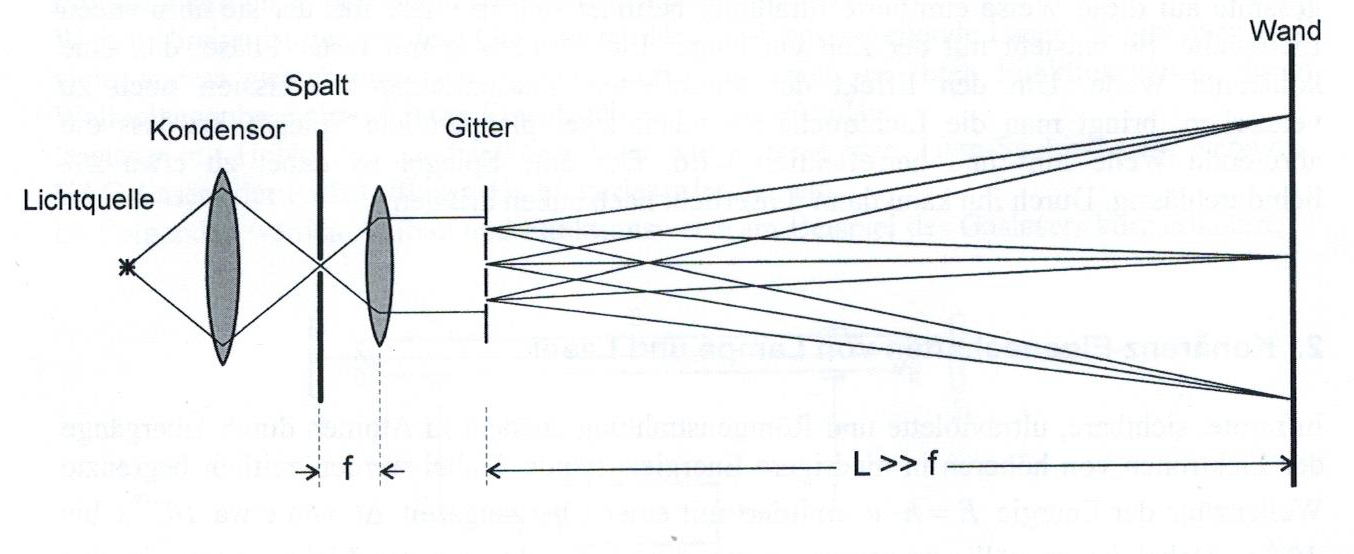
\includegraphics[scale=0.75]{Aufbau.PNG}
  \caption{Schaltbild zur Impedanzmessung (aus der Versuchsanleitung)}
  \label{fig:Aufbau}
\end{figure}

\subsection{Messwerte und Ergebnisse}
\begin{table}[H]
\captionof{table}{Messwerte für $U_{1}$, $U_{2}$ und daraus errechnete Werte für $I$ und $|Z|$.}
\begin{center}
\begin{tabular}{l|l|l|l|l}
Messung    & U\textsubscript{1} [V] & U\textsubscript{2} [V] & I [A] & |Z| [\textOmega] \\
\hline
Widerstand        & 0,55    & 0,45   & 0,00549   & 100,222 \\
Kondensator       & 1,2     & 0,305    & 0,00372   & 322,623 \\
Spule             & 1,2    & 0,26    & 0,00317   & 378,462 \\
Spule (digital)   & 1,16    & 0,27   & 0,00329   & 352,296
\end{tabular}
\end{center}
\label{tab:Gitter}
\end{table}
\subsubsection{Messung am Widerstand}
\subsubsection{Messung am Kondensator}
\subsubsection{Messung an der Spule}
\subsection{Fehlerrechnung}
\begin{align*}
\Delta R_{2} = \left| \frac{\partial R_{2}}{\partial U_{1}} \right| \Delta U_{1} + \left| \frac{\partial R_{2}}{\partial U_{2}} \right| \Delta U_{2} = \frac{R_{1}U_{2}}{U_{1}^2} \cdot \Delta U_{1} + \frac{R_{1}}{U_{1}} \cdot \Delta U_{2}
\end{align*}
\section{Impedanzmessung an einem unbekannten Zweipol)}

\section{Fazit}
\end{document}
